\emph{(This is a reproduction of a manuscript in preparation: }
Oliver Hoidn, Ryan Valenza, Gerald
T. Seidler, Alexander Ditter, William Holden, Evan
Jahrman, Samuel Vinko, Josh Kas, Fer Vila, Alison M.
Saunders, Luis Avila, Galen
O'Neil, Hae Ja Lee, and Bob Nagler,
Physical Review B, 2017
)



\begin{addmargin}[4em]{1em}
X-ray heating by x-ray free electron laser (XFEL) pulses is emerging as
an important method to create matter under extreme conditions. Many
prior reports of XFEL heating have focused on achieving extremely high
levels of ionization, and then have used advanced x-ray methods to with
the goal of evaluating the use of traditional plasma-theoretic
approaches to the resulting warm dense matter (WDM) where such
approaches may, or may not, be perturbatively applicable. Here, we adopt
a complementary strategy wherein we use more modest XFEL heating to
create more weakly ionized, `tepid' dense matter so as to investigate
the earliest stages of ionization and elucidate the boundaries of
applicability of traditional solid state physics ideas upon the
breakdown of its assumptions of, e.g., high electronic degeneracy and
coincident long range order of ion cores and valence charge density.
Specifically, we choose to study the early stages of XFEL heating of MgO
because of its large ground state bandgap, whose existence is a direct
consequence of such long range order, and because the rocksalt structure
of MgO holds special benefits in that its x-ray diffraction (XRD)
pattern can be used not only to look for changes in average ionization
of the unit cell but also for differential ionization between Mg and O
sites. We find an anomalously low onset for valence-level O 2p
ionization that requires the presence a large density of states within
the ground state band gap, despite the strong evidence that no ion core
motion has occurred during the x-ray pulse itself and despite the fact
that the O 2p ionization is still much too small for screening effects
to cause ionization potential depression. We propose that this may
instead be a consequence of the destruction of long-range order of the
electronic potentials due to site-disorder of the ionization, an effect
that would be an extreme manifestation of the Lifshitz tail effect that
is well-known in semiconductor physics.
\end{addmargin}



\section{I. Introduction}

The `warm dense matter' (WDM) regime resides in an important and
theoretically interesting middle-ground between the conditions typical
of high-pressure studies in condensed matter physics and those instead
of great interest to traditional plasma physics, where atoms are fully
ionized. WDM is defined by partial ionization, solid-like or higher
densities, substantial Fermi degeneracy (\(T \leq \ E_{F}\)), and values
for the plasma coupling parameter Γ of order unity or larger. \cite{koenig2005progress}
The collective properties of WDM---such as its equations of state (EOS),
opacities, and viscosities---are of fundamental importance in
geophysics, planetary and stellar astrophysics, and inertial confinement
fusion (ICF). \cite{atzeni2004physics}

However, the very intermediacy of WDM between condensed matter and
plasma physics conditions poses new challenges to fundamental
theoretical treatment of this state of matter because, on the one hand,
high degrees of ionization and incomplete Fermi degeneracy are poorly
treated even at a perturbative level by solid state physics electronic
structure methods and, on the other hand, the importance of the ion core
potentials, possible long-range order, and exchange interactions between
valence and core electrons pose unsolved challenges to adaptations of
theories intended for dense, more-completely ionized plasmas. In this
context, WDM created by electronic heating from x-ray free electron
laser (XFEL) pulses holds special promise, and has led to interesting
results for the electronic structure of matter at solid density and
relatively extreme degrees of valence-level ionization. \cite{rackstraw2015saturable, ciricosta2016measurements} Such
results are enabled not only by the creation of the WDM state by the
x-ray pulse but also by the experimental diagnostics enabled by those
same pulses, such as x-ray diffraction (XRD) and different
implementations of x-ray spectroscopies. \cite{chase2016ultrafast, yano2009x, mcneil2010x, chapman2011femtosecond}

However, we choose here a complementary paradigm for the scientific
opportunity provided by XFEL heating of dense matter. In contrast to
extreme ionization and inquiry into the perturbative persistence of
theories from the dense plasma physics literature, we instead seek to
finely interrogate the earliest stages of XFEL heating with an eye
toward seeing how far methods of solid state physics can find new,
extended relevance in a `tepid dense matter' regime where
plasma-theoretic approaches to electronic structure, such as screening
approaches to ionization potential depression, will not be applicable
because of choice of material or degree of ionization. In particular, we
report here a wide-angle XRD study of XFEL heating of the wide-bandgap
semiconductor MgO. The choice of method and material are intertwined and
are motivated by our overall scientific mission via two main
considerations.

First, a novel perspective on the use of elastic x-ray scattering, i.e.,
XRD, in the study of crystalline WDM has recently been presented by
Valenza and Seidler. \cite{valenza2016warm} While all early XRD studies of WDM were
performed in laser-shock studies where long-range crystalline order of
the target is destroyed, \cite{ma2013x} those authors instead address the
question of XRD from WDM created by heating of crystalline targets by
the extremely fast pulses created by x-ray free electron lasers (XFELs).
One key result of Valenza and Seidler is the large contribution to XRD
of the nominally `free' electrons for low-Z systems, but there are two
more overarching perspectives in that work that are more relevant for
the present study. To begin, XRD from crystalline WDM provides an
important testing ground for finite-T electronic structure theory,
giving direct measurement of the fundamental quantity predicted in DFT
approaches, i.e., the spatial distribution of charge density. For
example, for low-Z systems, finite-T studies of XRD might give an
especially salient inquiry into exchange functional effects under
intermediate degeneracy of the unbound electrons. \cite{karasiev2012comparison, dufty2011scaling, sjostrom2012temperature} Next, and
of greater relevance here, XRD from a WDM state where the ion cores are
at least effectively stationary is a rich experiment that, through the
careful choice of target material crystal structure, can be designed to
have far higher information content about microscopic parameters, such
as species-specific ionization states, than has been the case in studies
of disordered WDM or simple elemental metal targets. In particular, we
show here that species-specific ionization state sensitivity can be
obtained by judiciously selecting a crystalline compound whose
diffraction peaks express a combination of destructive and constructive
interference between different atomic sites in the unit cell. The
rock-salt structure taken by MgO is a classic textbook example of
exactly this effect. Of relevance here, the (200) and (220) Bragg peaks
have perfect constructive interference between charge density at the Mg
and O sites in the unit cell, whereas the (111) peak instead has perfect
destructive interference.

Second, the choice of MgO is particularly appropriate here because of
its ground state electronic structure. MgO is a strongly ionic, very
wide-band gap insulator. As such, unlike with an elemental metal target
such as Al or Cu, the valence electronic charge density is quite
spatially localized and has a strong contribution to the XRD that must
rapidly change upon ionization. For example, prior study of strongly
electronically excited KH\textsubscript{2}PO\textsubscript{4} using
optical bandgap excitation and XRD diagnostics found clean signatures of
the resulting changes in real space charge distribution. In the present
case, with an ionic rather than molecular crystal, it is important to
recognize that the wide bandgap of MgO, 7.8 eV, is a special
manifestation of the ground state crystalline symmetry and long-range
order of both the atomic positions and the local electronic structure.
As such, the large ground-state band gap provides a special, potentially
very sensitive, opportunity to see the initial consequences of the
breakdown of the ground-state symmetries.

With background complete, we summarize our results. During the
single-shot studies, where heating and diffraction occur simultaneously,
we find no signatures of long-range lattice disorder, such as either
Debye-Waller or `Bragg gating' effects, across a range of energy
deposition densities reaching 150 eV per unit cell. However, we measure
a monotonic rise in normalized intensity of the (111) peak of MgO with
increasing XFEL flux density. This effect is the fully expected
signature of a loss of destructive interference within the MgO unit cell
as the valence electrons progressively delocalize from their O
2\emph{p}-like ground state locations. This is an observation of
short-range, purely electronic charge reorganization in a solid-density,
partially-ionized plasma that constitutes an initial demonstration of
the general type of `warm dense crystallographic' effect predicted by
Valenza, et al. \cite{valenza2016warm} The observed onset for strong O 2\emph{p}
ionization is, however, anomalously low when compared to constraints
that would be imposed by the large ground-state band gap of nearly 8 eV.
We propose that the site-disorder of ionization that is a hallmark of
x-ray heating is likely introducing a significant density of states
within the ground state band gap, thus giving a new mechanism,
independent of, e.g., traditional inonization potential depression
(IPD), for enhanced ionization effects in WDM. Such `Lifshitz tails' are
well known in the theory of semiconductor physics but have not
previously been discussed in the context of WDM. Although the lack of
local thermal equilibrium (LTE) in the present study limits the utility
of comparisons to theory, the experiment validates wide-angle XRD as an
effective probe of local real-space electronic reorganization in
crystalline warm dense matter. It thus presents the appealing prospect
of future XRD studies on XFEL-heated WDM and solid-density plasmas
designed to empirically constrain DFT-based predictions of
finite-temperature electronic structure, especially for experiments
performed using two-color x-ray pump, x-ray probe methods where many
limitations of the present study will be ameliorated.

We continue as follows. First, in section II we describe experimental
methods. In section III we discuss approaches for modeling variations in
the Bragg diffraction signal as a consequence of XFEL heating. This
includes ground-state, molecular, density functional theory, and
species-by-species radiative combination calculations. In section IV we
present and discuss experimental and modeling results, the most
consequential of which is that the presence of valence disorder
substantially complicates interpretation of WDM structure by
invalidating ground state-based treatments of the electronic structure
and providing a new route for effective enhancement of ionization
effects that is specific to crystalline dense plasmas.. Finally, in
section IV we conclude and discuss future directions.

\section{II. Experimental Methods}

\subsection{II. A. Experimental Details}

The experiment was performed at the matter of extreme conditions (MEC)
endstation of the Linac Coherent Light Source (LCLS), where XFEL pulses
were used to excite MgO samples consisting of a 100 nm-thick layer of
PMMA with embedded MgO nanoparticles (Sigma Aldrich, typical size 50 nm)
on an 8 µm-thick polyimide substrate. We used self-amplified stimulated
emission (SASE) pulses of 45 fs mean duration, average pulse energies of
2 mJ, and a nominal x-ray energy of 9 keV. Variations in the mean photon
energy of each pulse are monitored by a downstream dispersive
spectrometer. We controlled the flux density incident on the sample via
a stack of Be lenses, with which we varied the focal spot diameter of
XFEL pulses at the sample position from 2 to 60 µm; these diameters were
determined using an ablative imprint method to measure the spatial
profile of the focused XFEL beam.  Using the full available
range of focal spot sizes and the unattenuated beam, we obtained
incident flux densities ranging from 30 to 2000 J/cm\textsuperscript{2}.

During data collection the sample's position was rastered at a rate of
100 µm between the XFEL pulses, whose repetition rate was 120 Hz. At
every XFEL pulse the Bragg scattering signal was collected and read out
from a quad CSPAD solid state detector having 800 x 800 resolution and a
pixel pitch of 100 µm. \cite{hart2012cspad} The 8 x 8 cm\textsuperscript{2}
active area of the detector subtended the range of scattering angles
from 10 to 58 degrees, encompassing the (111), (200), and (220) Bragg
reflections of MgO (located at 33.5, 38.8, and 55.9 degrees,
respectively, for 9 keV incident photons).

\subsection{II.B. Data Reduction and Analysis}

Several steps of processing and event selection were performed prior to
generating powder diffraction patterns. For each event the quad CSPAD
readout was corrected by subtracting pixel pedestals (measured using
previously-collected dark exposures) as well as common-mode noise in
each of the detector's 16 individual tiles. \cite{hart2012cspad} Due to the small
number of photon hits in a single shot residual ADC noise often
dominated the Bragg scattering signal. To address this we made use of a
standard component of the analysis pipeline for CSPAD data in low-photon
count rate experiments at the LCLS, such as macromolecular imaging and
crystallography, which identifies clusters of spatially-concentrated
signal resulting from x-ray photon hits, rejecting the output of
noise-dominated pixels. \cite{damiani2016linac}

For each LCLS pulse a powder diffraction pattern is generated from the
quad CSPAD frame by the summation of elliptically-shaped strips of
pixels at equal scattering angle. The mapping of pixel coordinate to
scattering angle is calculated from the CSPAD's location and orientation
relative to the sample and incident XFEL beam; this geometry is in turn
obtained from the conic section parameters of powder diffraction peaks
in data from a known reference material measured in the same
source-detector geometry. After generation of a powder pattern, two
corrections are made. First, the each peak is shifted to correct for
angular offsets caused by imperfect flatness of the sample substrate and
also event-to-event jitter in the mean photon energy of the XFEL.
Second, a linear fit is made to the background of each peak, and this
background is subtracted from the peak signal. The signal-to-background
ratio for this peak is then computed by comparison of the background
level derived from the linear fit to a simple integration of the
background-subtracted peak. Events in which any of the peak
signal-to-background ratios fall below a threshold (chosen to be 0.2)
are rejected in subsequent summation over data from multiple events.

Bragg peak scattering intensity is the most significant derived quantity
from each powder pattern in this study, but its estimation requires
correcting the effect of variations in the total scattering signal
caused by sample non-uniformity and temporal variation of the XFEL pulse
energy. The latter contribution can be corrected using direct
measurement of incident pulse intensities available from an upstream
nitrogen detector; for comparison of Bragg peak intensities at different
flux density values, however, we normalize each pattern to the integral
intensity of its (200) peak in order to control for variations in sample
thickness, or fluctuations in nanoparticle volume in the beam, such as
from nonuniform aggregation..

\section{III. Modeling Methods}

Finally, the relationship between the incident flux density and the
resultant energy density in the MgO nanoparticles requires some care.
The small (100 nm) sample thickness requires that a significant portion
of higher-energy electrons created in the relaxation cascade following,
e.g., primary photoionization of the Mg 1s orbital, will necessarily
escape into the surrounding low-Z substrate and surrounding binder,
causing a reduction in the density of \emph{locally deposited,} versus
absorbed, energy from the incident XFEL pulse. This effect has recently
been discussed in detail, and proposed to be especially important for
the design of XFEL x-ray heating targets. \cite{hoidn2017nonlocal} In the present case,
using the methods described in \cite{hoidn2017nonlocal} we use PENELOPE to perform Monte
Carlo simulations for 9 keV incident photons striking a target
consisting of a 50-nm thick MgO layer clad with graphite, where graphite
is taken as representative of carbonaceous binder and substrate
materials. This simulation implements particle-tracking simulation of
electron showers in which elastic scattering differential cross sections
are calculated from partial-wave solutions to the Dirac equation, while
inelastic interactions (involving both impact ionization and collective
excitations) are represented using a modified version of Liljequist's
`delta-oscillator' generalized oscillator strength (GOS) model. \cite{hoidn2017nonlocal}

The average energy deposited per unit cell is then calculated on the
basis of the incident pulse energy, the focal spot size, standard (cold)
cross sections for x-ray absorption, which greatly dominates Compton and
elastic scattering, and the above correction. This calculation is an
upper bound, in that it assumes that long-wavelength electronic
excitations, e.g., plasmons, are a minor contributor to the energy
distribution at any moment in the relaxation cascade and will have
decayed to simple electron-hole excitations during the time duration of
the pulse.

To model the dependence of the XRD signal on the electronic
configurations of the Mg and O ions we use the Hartree-Fock code of
Cowan \cite{abdallah1988theoretical} to calculate the atomic form factors of Mg and O
decomposed by subshell. The crystal's structure factor is subsequently
calculated as a sum over basis atoms and subshells; i.e.,

\(S\left( \overrightarrow{Q} \right) = \sum_{j}^{}{\sum_{n,l}N_{n,l}f_{j,n,l}\left( Q \right)e^{- i\ \overrightarrow{Q} \bullet \overrightarrow{r_{j}}}\ },\)
(1)

where \(f_{j,n,l}\left( Q \right)\) is the atomic form factor of the
subshell \(n,l\) of the jth species, where \(n\) and \(l\) are principal
and orbital angular momentum quantum numbers, and \(N_{n,l}\) is the
subshell's population. The intensity of a given Bragg reflection
(neglecting Debye-Waller quenching and the geometric dependence of
scattering by a powder of crystallites) is then obtained by evaluating
\(S\left( \text{h\ }\mathbf{a}_{\mathbf{1}} + \ k\ \mathbf{a}_{\mathbf{2}}\mathbf{+ \ }\text{l\ }\mathbf{a}_{\mathbf{3}} \right)\),
where \(\mathbf{a}_{\mathbf{1}}\mathbf{,\ }\mathbf{a}_{\mathbf{2}}\) and
\(\mathbf{a}_{\mathbf{3}}\) are the basis vectors of the reciprocal
lattice and \(h\), \(k\) and \(l\) are Miller indices. Following
standard practice in plasma physics modeling, we treat ionization of
atomic electrons as a uniform (real-space) smearing of free electrons;
thus, ionization of an atomic orbital simply corresponds to reduction of
its weight \(N_{n,l}\).

In the high-energy density regime, defined as having mean temperatures
above 2 eV, we simulated the temporal evolution of the MgO charge state
distribution (CSD) over the course of an XFEL pulse using a variant of
the collisional radiative code SCFLY that Vinko et al. have modified to
self-consistently support elemental mixtures. \cite{ciricosta2016measurements} The code
implements a local density-based treatment of continuum lowering that
Vinko et al. have demonstrated accurately reproduces experimental
ionization potential shifts at high charge states in several
solid-density plasma mixtures. Unlike other collisional radiative codes,
SCFLY models the plasma's free electron energy density self-consistently
with respect to XFEL heating and interaction with ions (e.g. impact
ionization and Auger decay). Its principal caveat in the current
setting, where the plasma is heated via photoexcitation by photons with
energies far above the absorption edges of Mg and O, is its assumption
of an instantly-equilibrating thermal distribution of free electrons.
{[}22{]}

Our inputs to SCFLY were the sample composition and XFEL photon energy,
flux density, and temporal profile (which we took as a Gaussian with a
45-fs FWHM duration); the main outputs were temporal profiles of the
charge state populations of Mg and O during the XFEL pulse. With the
help of a simplifying approximation (discussed in section III below)
that relates Mg and O charge states to 2p ionization, we used the AFF
ionization model to obtain predicted Bragg peak intensity ratios for
each simulated incident flux density.

In the low-energy density regime we instead adopt three alternate models
that capture aspects of the condensed phase physics under contrasting
assumptions and limiting conditions. First, we use the Vienna ab-initio
Simulation Package (VASP) \cite{hafner2008ab}, a density functional theory (DFT)
code, to compute the X-ray diffraction signal at finite temperature
using the charge distributions of Kohn-Sham eigenstates populated by
Fermi-Dirac Statistics. The relation between temperature and deposited
energy density is derived from the zero-temperature density of states of
MgO, which we compute using the code FEFF. \cite{ankudinov1998real} Under this model it
is assumed that the potential landscape and density of states are not
significantly altered by finite-temperature redistribution of charge.
Additionally, the presence of local thermal equilibrium is implicit.

Second, we take a simplified picture of XFEL heating where all energy
deposited in the MgO sample contributes to excitation of O 2p states.
Departing from the ground state density of states (DOS), we assume that
the energy required to delocalize an O \emph{2p} electron is equal to
the band gap, 7.8 eV. Under these assumptions a given XFEL dose
therefore generates a known amount of O 2p ionization; from this, the
AFF model is used to calculate the resulting XRD response. We term this
approach the ground state model.

Third and finally, we consider the limit in which perturbation of the
electronic structure creates a large density of states in the band gap
and the O \emph{2p} ionization potential is determined by local
interactions alone. In this molecular model we approximate the
ionization potential of O\textsuperscript{2-}, embedded in a dielectric
background mimicking bulk MgO, using a delta SCF (self-consistent field)
calculation. \cite{neese2006critical} This approximation yields an ionization potential
of 1.9 eV, from which the XRD response can be calculated in the same
fashion as in the ground state model

\section{IV. Results and Discussion}

\begin{figure}[h] \label{cm2image1}
\caption{
(a): Experimental intensity of the (220) Bragg peak
from a sample of MgO simultaneously heated and probed by 45-fs duration
XFEL pulses, as a function of XFEL energy deposited per MgO unit cell,
with no normalization across individual data points. (b): Equivalent
data for the (200) peak. (c): Experimental intensities of the (111)
peak, compared to several models. Each experimental data point is
normalized by (1) its intensity at minimum flux density and (2) the
(200) peak intensity. For each of the four displayed models, the shaded
region corresponds to the locus of possible curves once the loss of
in-sample energy deposition due to nonlocal heat transport by hot
electrons is accounted for. See the text for discussion.
}
\centering
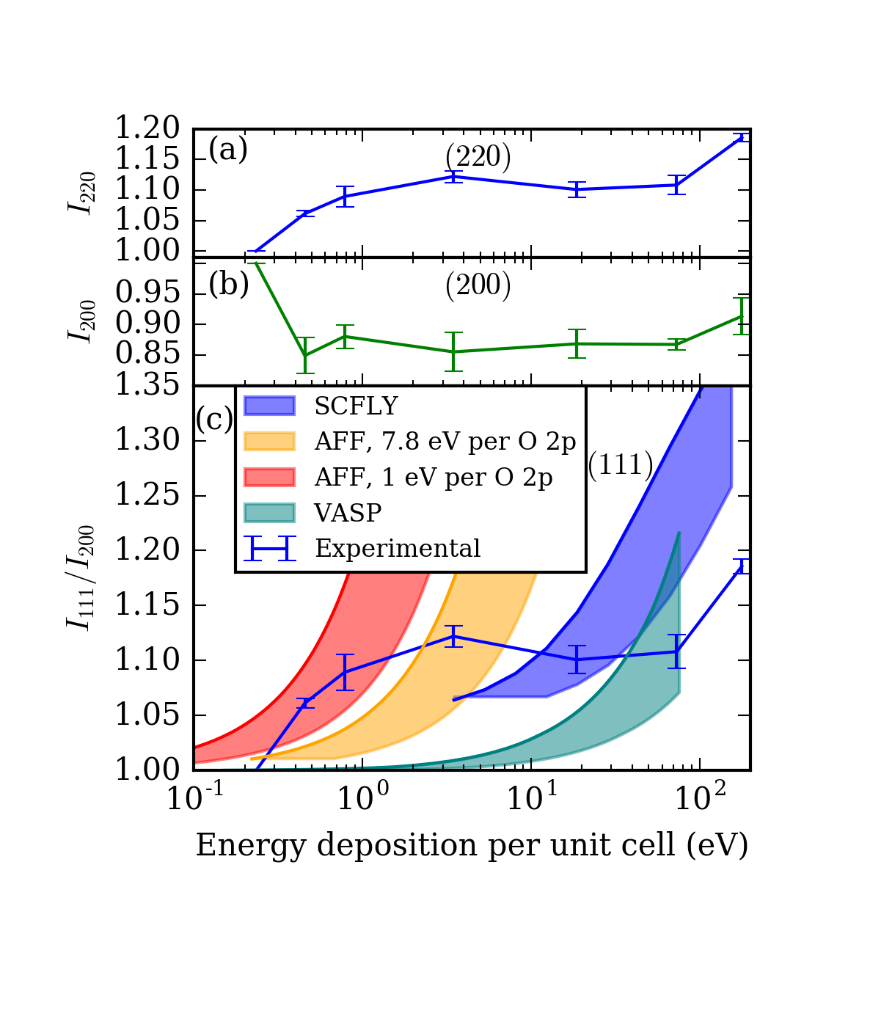
\includegraphics{MgO_2.7.docx1503027860/media/image1.png}
\end{figure}

To begin, in Fig. \ref{cm2image1} (a), we show the experimentally measured intensity
of the MgO (200) peak as a function of energy deposited per MgO unit
cell. The \textasciitilde{}15\% scatter in the observed scattering
intensity upon increasing excitation is explained as being due to
variations in MgO nanoparticle content across different regions of the
sample. Consequently, our first result is clear: the MgO nanoparticles
remained substantially, and possible completely, crystalline for the
duration of the XFEL pulse. There is no evidence for `Bragg-gating' or
other self-limiting diffraction signals that are known to be important
in the context of macromolecular crystallography at XFELs. \cite{caleman2015ultrafast}


In Fig. \ref{cm2image1} (b) we plot the normalized experimental intensity of the (111)
and (220) Bragg peaks of MgO as a function of incident flux density
(together with curves for several models, which we discuss below).
Specifically, for each Bragg peak, the entire curve is normalized to the
intensity of the ``cold'' (lowest-flux density) dataset and each
individual data point is normalized to the (200) peak intensity for the
corresponding flux density. The normalization to the intensity of the
(200) peak helps to remove fluctuations in diffracted intensity due to
sample thickness nonuniformity. We hereafter refer to intensities
normalized in this fashion, for a given peak (hkl), as
\(I_{\text{hkl}}/I_{200}\). Displayed error bars are estimated
systematic errors due to background subtraction and peak integration;
counting statistics-derived errors are negligible. The most salient
feature is a 20\% rise in the relative intensity of the (111) peak
between the lowest and highest flux densities. In contrast, the relative
intensity of the (220) peak fluctuates but does not display a monotonic
progression. The behavior of both curves---and in particular the rise in
relative intensity of the (111) peak---is strongly at odds with the any
Bragg peak quenching that would result from a Debye-Waller thermal-like,
uncorrelated, increase in the mean squared displacement of atoms from
their lattice sites. The absence of any such signature further supports
the crystallinity of the heated target and the isolation of the
deposited energy in the electronic, rather than lattice, degrees of
freedom.

\FloatBarrier

A first step toward understanding the increase in relative intensity of
the (111) Bragg peak comes from consideration of the ground-state x-ray
crystallography of MgO. MgO's rock salt-type crystal structure consists
of two interpenetrating FCC lattices of Mg and O, with one of the
lattices shifted by half of the FCC lattice constant in the direction of
one of the lattice basis vectors. This has consequences for the
dependence of the (200), (111), and (220) Bragg peak intensities on the
characteristics of the ions on the two sites in the primitive basis, as
is frequently discussed in introductory texts. \cite{kittel2005introduction} In particular,
the (200) and (220) peaks result from perfect constructive interference
between the two unit cell sites while the (111) peak, on the other hand,
instead has perfect destructive interference between the two unit cell
site. The nominal ground-state ionic species of MgO,
Mg\textsuperscript{2+} and O\textsuperscript{2-}, have identical
electron configurations and have only very slightly different ionic form
factors for x-ray scattering as a secondary consequence of the different
nuclear potentials on the spatial extent of the electronic
wavefunctions. This offers an explanation for the small ground-state
intensity of the (111) Bragg peak, as well as for its monotonic rise
with increasing incident x-ray flux: as temperature increases electrons
of the weakly-bound O 2p orbitals are ionized at a higher rate than
those of Mg semi-core 2p orbitals, increasing the dissimilarity of the
form factors of the O and Mg ions.

This relationship is illustrated by Fig. \ref{cm2image2}, which shows
\(I_{111}/I_{200}\) as a function of O 2\emph{p} and Mg 2\emph{p}
population under the AFF ionization model presented in section II. Three
curves denoting different scenarios for the electronic configuration of
Mg and O following x-ray heating are indicated in Fig. \ref{cm2image2}b, and the
corresponding Bragg peak intensity progressions are plotted in Fig. \ref{cm2image2}b.
First, trajectory (i) corresponds to progressive ionization of the O 2p
electrons with a fixed (ground state) population of Mg 2\emph{p}
electrons; it encompasses possible states of the x-ray excited system
following relaxation of all deeply-bound Mg 2\emph{p} holes. Along
trajectory (i), removal of O 2p charge density causes the (111) Bragg
peak intensity to increase monotonically due to reduction in the O
electrons' cancellation of the Mg charge density's scattering amplitude.
Conversely, on trajectory (ii) only Mg 2\emph{p} electrons are ionized;
noting that the Mg K shell dominates the photoelectric cross section of
MgO at hard x-ray energies, this corresponds to the locus of possible
initial states following instantaneous x-ray ionization. In this case,
ionizing the Mg 2p orbitals (starting from the ground state) reduces the
magnitude of the total scattering amplitude until total destructive
interference is reached before the scattering factors differ again as Mg
2\emph{p} ionization continues. The resulting intensity progression for
case (ii) in Fig. \ref{cm2image2}b therefore has a local minimum (located at an Mg
2\emph{p} population of approximately 3.5 electrons). Finally,
trajectory (iii) represents an intermediate scenario wherein the levels
of O and Mg 2\emph{p} ionization are (artificially) equal. Here, the
dominant effect is a slow decrease in intensity due to uniform reduction
of the scattering amplitude contributions of all 2p electrons in the
unit cell.

\begin{figure}[h] \label{cm2image2}
\caption{
Dependence of
\(I_{111}/I_{200}\)
on population of the \emph{2p} orbitals of
\(\text{Mg}^{2 +}\)
and \(O^{2 -}\), according to an atomic form factor (AFF) based model of
ionization. This ratio reaches a maximum factor of 13.8 times the
unperturbed value at full ionization of the O 2p electrons.
}
\centering
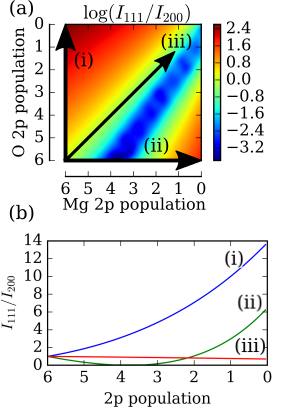
\includegraphics{MgO_2.7.docx1503027860/media/image2.png}
\end{figure}

Referring back to the results of Fig. \ref{cm2image1}c
for \(I_{111}/I_{200}\), we see a more gradual enhancement than is the case
for a thermalized system with only O 2\emph{p} ionization and there is
no evidence of initial decreases for states dominated by Mg 2\emph{p}
ionization. The resulting qualitative conclusion is then a trajectory
intermediate between (i) and (ii), where any theoretical treatment will
need to include both the lifetime of the Mg 2\emph{p} core holes during
the x-ray excitation and also the presence and significant, if
incomplete, thermalization of O 2\emph{p} valence-level electrons.
Because of the counteracting effects of O and Mg \emph{2p} ionization in
this regime, the value of \(I_{111}/I_{200}\) does not fully constrain
the extent of either O or Mg \emph{2p} ionization. Trajectory (i)
nevertheless delimits the minimum extent of O \emph{2p} delocalization
as a function of \(I_{111}/I_{200}\); the largest experimental value of
\(I_{111}/I_{200}\) corresponds to an O \emph{2p} ionization level of at
least 5 \%.

Hence, predicting the consequences of single-pulse XFEL heating on XRD
requires separate calculation of an average of the probed Mg and O
ionization states ---both temporal (over the duration of an XFEL pulse)
and spatial (over all probed unit cells). We begin with the low-energy
limit. In the regime where energy deposition per unit cell is less than
1 eV, condensed matter physics and the details of valence-level
electronic structure should be dominant. For example, prior work on the
XRD from KH\textsubscript{2}PO\textsubscript{4} after strong optical
excitation from the valence band to the conduction band could be
well-interpreted in the general arena defined by the ground-state
electronic structure of the crystalline phase. \cite{zamponi2012ultrafast}

Here, the absence of local thermal equilibrium (LTE) is a challenge for
modeling fs-scale electronic reorganization in the 0.1-1eV temperature
regime because---unlike in the plasma limit, where the atomic kinetics
are unambiguous (modulo treatment of the ionization potential
depression)---there is a lack of established frameworks for calculating
the time-evolved electronic structure. We thus forgo \emph{ab initio}
simulation and take a simple assumption of proportionality between the
density of deposited energy and the level of O 2\emph{p} ionization.
Under this assumption, we then consider two idealized bounds on the
excitation kinetics.

First, we consider the case where the ground state electronic structure
is taken as a static venue that is unperturbed by even relatively high
levels of ionization, i.e., where the energy needed to excite an O 2p
electron is equal to the band gap of MgO, \(E_{g}\) = 7.8 eV no matter
the level of O 2\emph{p} ionization. The results of this naïve ground
state model are shown as a shaded region (orange) with label AFF 7.8 eV
in Fig. \ref{cm2image1} Under this condition, and defining \(\rho_{E}\) as the
density of deposited XFEL energy, it follows that \({\rho_{E}/E}_{g}\)
is an upper bound on the concentration of O 2\emph{p} excitations (i.e.,
corresponding to all XFEL energy coupled into O 2\emph{p} excitation).
The yellow shaded region of Fig. \ref{cm2image1} shows the ground state model's
predicted intensity progression of the (111) Bragg reflection as a
consequence of a density of deposited energy equal to
\({\rho_{E}/E}_{g}.\) The measured onset of the (111) peak intensity's
rise is much delayed compared to the model's prediction, from which we
can infer that the experimental level of O 2\emph{p} delocalization is
significantly higher than that allowed by the ground state density of
states of MgO -- in other words, there must be a plethora of states in
the band gap that occur as a consequence of the x-ray excitation, even
while periodicity of the ion-core locations is preserved. This
inconsistency is corroborated by comparison of the experimental
progression with a more advanced calculation of the same ilk, a
finite-temperature DFT-based calculation, which also fails to reproduce
the (111) peak's early rise (teal region in Fig. \ref{cm2image1}, labeled VASP).

Second, as an alternative bounding case, one may consider an isolated,
atomic O\textsuperscript{2-} in an MgO-like dielectric background
results in a much lower calculated ionization threshold of 1.9 eV. This
limit would be representative of a complete breakdown of any band-like
effects. The general, quadratic shape is still shown (color, label in
overestimate of the onset for O 2\emph{p} ionization. Hence, the
dilute-plasma limit, modified only by ion-pairing for local neutrality,
has omitted too much of the condensed phase physics.

\FloatBarrier

Given the above discussion, the question then arises as to possible
explanations for the observed enhancement of O 2\emph{p} ionization at
lower incident energy densities. Prosaically, some part of this effect
may be due to our choice of nanophase material. Unsurprisingly, the
finite size of MgO nanostructures manifest surface states with energies
inside the ground state band gap.  However, the magnitude of the
present effect requires a more intrinsically bulk-like behavior. Though
the effect superficially resembles ionization potential depression
(IPD), conventional models of IPD inevitably fail in the low-energy
density regime because they treat variations in the continuum level as a
consequence of screening, with dependence only on the average ionization
and ion density of a plasma, quantities that are showing only very small
changes here compared to that needed for substantial changes in
screening. \cite{ciricosta2016measurements, vinko2014density} Here, the key physics may instead be the fact that
while long-range structural order persists, long-range \emph{electronic}
order has been significantly weakened by the site-randomness of
ionization on both the O sites (by valence-level ionization) and on the
Mg sites (due to the long lifetime of Mg 2p vacancies created during the
relaxation cascade).. It is known that site disorder in an otherwise
perfectly crystalline solid (for instance lattice vacancies, impurities,
or, as in our case, randomly-distributed electron vacancies) can
introduce localized states with energies inside the band gap, a spectral
phenomena referred to as Lifshitz tails. \cite{nieuwenhuizen1989trapping} One particularly
celebrated example of this is Anderson delocalization. \cite{de1998delocalization} The
possibility that this classic idea in solid state physics may find new
application in dense plasma physics is an interesting result that can be
further interrogated with, e.g., large-cluster quantum chemistry
calculations or with other real-space DFT methods where site disorder of
ionization state can be directly manipulated.

We now turn our attention to high energy deposition densities in Fig. \ref{cm2image1}.
In this regime, treatment of the interaction between atomic and free
electrons, which gives rise to plasmas physics effects such as continuum
lowering, becomes necessary. The above atomic and solid state treatments
become inappropriate---even for the purpose of establishing rough bounds
on the concentration of excitations---and we instead turn to
time-resolved collisional radiative simulation.

\begin{figure}[h] \label{cm2image3}
\caption{
Electronic temperature evolution during an XFEL pulse
simulated by the radiative collisional code SCFLY. The incident XFEL
photon energy and flux density are 9 keV and 2 x 10\textsuperscript{4}
J/cm\textsuperscript{2}, respectively. The dashed line represents the
temporal profile of the incident XFEL pulse.
}
\centering
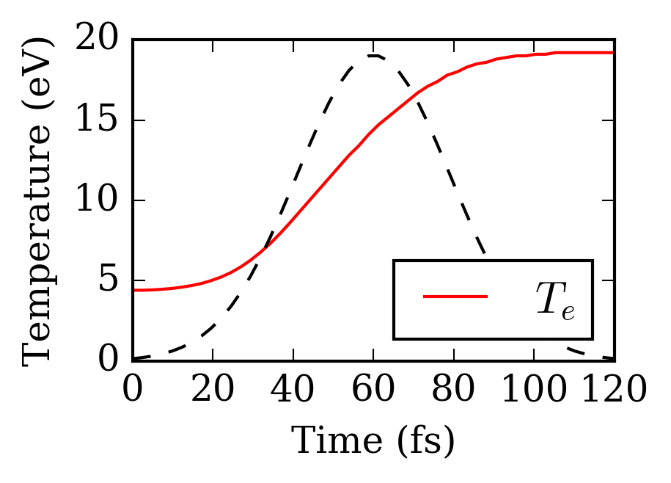
\includegraphics{MgO_2.7.docx1503027860/media/image3.png}
\end{figure}

\begin{figure}[h] \label{cm2image4}
\caption{
Evolution of the mean charge states Mg and O of during
an XFEL pulse simulated by the radiative collisional code SCFLY. The
incident XFEL photon energy and flux density are 9 keV and 2 x
10\textsuperscript{4} J/cm\textsuperscript{2}, respectively. The dashed
line represents the temporal profile of the incident XFEL pulse.
}
\centering
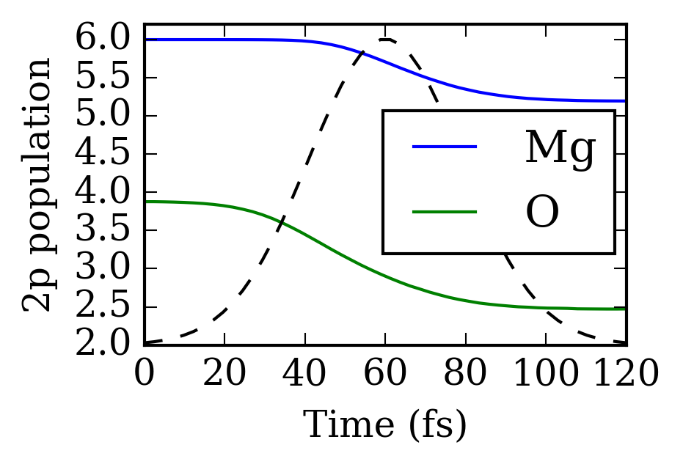
\includegraphics{MgO_2.7.docx1503027860/media/image4.png}
\end{figure}

The principal outputs of such a simulation are temporal evolutions in
electron temperature and atomic species charge states. Figs. \ref{cm2image3} and \ref{cm2image4}
display these data for simulated XFEL heating of an MgO target,with an
incident XFEL intensity equal to the highest experimental value using
the code SCFLY. Notably, the charge state distribution is strongly
athermal: the difference between the initial and final Mg 2p population
levels is 0.8 electrons, which exceeds the equilibrium ionization level
corresponding to the final temperature of 19 eV by a large factor. One
reason for the lack of LTE is readily apparent. The lifetime of Mg 2p
holes is large compared to the 45 fs XFEL pulse duration \cite{keski1974total, fuggle1992unoccupied} and
the simulated free-electronic temperatures are far below the Mg 2p
binding energy. Consequently, the production of Mg 2p holes will be
dominated by rates of 2p and 1s photoionization and electron impact
ionization during the XFEL pulse.

\FloatBarrier

The low value of the free electronic temperature relative to the
\emph{K} shell binding energies of O and Mg allows a simplification in
application of the AFF ionization model to the output of SCFLY. Because
only the 2\emph{p} orbitals of Mg and O are substantially ionized, the
charge state of each species uniquely determines its electronic
configuration under Eq. 1. Progressions of Mg and O charge states (or,
equivalently, Mg and O 2\emph{p} populations) therefore contain
sufficient information to compute Bragg peak intensities using the AFF
model. Fig. \ref{cm2image1}c shows the output of the resulting SCFLY-based XRD
calculation evaluated over the full range of flux densities simulated
with SCFLY At high flux density agreement between the experimental Bragg
peak intensity data and SCFLY-based model is poor but shares a
qualitative features with the experimental data, namely a rapid rise in
intensity of the (111) peak beyond a 5 eV per unit cell energy
deposition.

A few explanations can be proposed for the plateau in
\(I_{111}/I_{200}\) at higher flux densities, although additional work
will clearly be needed. First, the population of excitons may saturate
at high flux densities due to dependence on the exciton recombination
rate on deposited energy density. A robust modeling of the energy
relaxation cascade that includes both long-wavelength excitations
(plasmons) and also point-like excitations (ionization) would be needed
to better understand such a proposition. Alternatively, a reduction in
the rate of ionization may arise from an increase in the 2\emph{p}
ionization potential as more electrons enter excited states (though this
effect competes with IPD).

\section{V. Conclusion and Future Directions}

We have explored the use of single hard x-ray XFEL pulses to
simultaneously create and probe crystalline WDM via wide-angle x-ray
diffraction. We present experimental results on the consequences of XFEL
heating on the electronic structure of MgO as a function of deposited
energy density, using a Hartree-Fock orbital-based model of ionization
to infer electronic subshell populations from experimental Bragg peak
intensities. We find that the experimental XRD signal is a sensitive
measure of charge reconfiguration, allowing inference of valence
ionization levels with a precision of under 0.1 electrons per unit cell.
This sensitivity is in large part contingent on the structure of the
system chosen: the odd-numbered Bragg reflections of MgO exhibit
near-destructive interference in the ground state with a rapid,
easily-measurable increase in intensity upon delocalization of electrons
in the highest occupied molecular orbital (HOMO).

The experimental data shows a rapid delocalization of O 2p electrons at
deposited energy densities per unit cell far below the 7.8 eV band gap
of MgO, which constitutes evidence for the creation of excitations
within the ground state band gap. Significantly, we find no indication
of a loss of long-range order in the positions of ion cores; we propose
that the presence of states in the ground state band gap is instead a
consequence of long-range disorder in the electric potential caused by
ionization-derived site disorder.

Theoretical interpretation of the data is made difficult by the lack of
LTE (a consequence of the presence of long-lived Mg 2p holes), which
renders comparison to finite-temperature DFT calculations impossible.
Consequently, future experiments will aim for a closer approach to local
thermal equilibrium in the probed system. One way of achieving this will
be by studying systems free of long-lived excitations like those of the
Mg 2p core hole that complicate the present analysis. Heavier rock-salt
materials such as KCl are promising candidates as they exhibit
shorter-lived \emph{p} vacancies than MgO while sharing its most
important features: namely, a large band gap and a diffraction signal
with high sensitivity to site-specific charge delocalization. A closer
approach to local thermal equilibrium can also be achieved by using
time-resolved measurements under two-color pump-probe operation of the
XFEL: specifically, a sufficient delay between pump and probe provides
time for thermalization of electronic degrees of freedom. An additional
benefit of two-color pump/probe configurations is the ability to
interrogate temporally uniform states, instead of integration over a
sample's evolution during XFEL stimulation (as is the case with
single-pulse simultaneous pump/probe). Given the present hypothesis of
strong changes in the density of states within the ground-state bandgap,
it is also interesting to consider x-ray pump studies with optical (or
UV) probe to directly evaluate changes to the electronic energy
landscape on the energy scale of the band gap and ionization thresholds.
In future studies it may be worthwhile, finally, to study non-rock salt
compounds that similarly manifest a combination of destructive- and
constructive-interference diffraction peaks. One possibility is layered
binary dielectrics, in which one would expect strong sensitivity to
interplanar charge reorganization effects.


%\section*{References}
%
%{[}1{]} M. Koenig \emph{et al.}, Plasma Physics and Controlled Fusion
%\textbf{47}, B441 (2005).
%
%{[}2{]} S. Atzeni and J. Meyer-ter-Vehn, \emph{The Physics of Inertial
%Fusion: BeamPlasma Interaction, Hydrodynamics, Hot Dense Matter} (Oxford
%University Press on Demand, 2004), Vol. 125.
%
%{[}3{]} G. Faussurier, C. Blancard, P. Cossé, and P. Renaudin, Physics
%of Plasmas \textbf{17}, 052707 (2010).
%
%{[}4{]} D. Rackstraw \emph{et al.}, Physical review letters
%\textbf{114}, 015003 (2015).
%
%{[}5{]} O. Ciricosta \emph{et al.}, Nature Communications \textbf{7},
%11713 (2016).
%
%{[}6{]} A. Höll \emph{et al.}, High Energy Density Physics \textbf{3},
%120 (2007).
%
%{[}7{]} B. E. Warren, \emph{X-ray Diffraction} (Courier Corporation,
%1969).
%
%{[}8{]} J. Yano and V. K. Yachandra, Photosynthesis Research
%\textbf{102}, 241 (2009).
%
%{[}9{]} B. W. McNeil and N. R. Thompson, Nature photonics \textbf{4},
%814 (2010).
%
%{[}10{]} H. N. Chapman \emph{et al.}, Nature \textbf{470}, 73 (2011).
%
%{[}11{]} R. A. Valenza and G. T. Seidler, Physical Review B \textbf{93},
%115135 (2016).
%
%{[}12{]} T. Ma \emph{et al.}, Physical Review Letters \textbf{110},
%065001 (2013).
%
%{[}13{]} V. V. Karasiev, T. Sjostrom, and S. Trickey, Physical Review E
%\textbf{86}, 056704 (2012).
%
%{[}14{]} J. W. Dufty and S. Trickey, Physical Review B \textbf{84},
%125118 (2011).
%
%{[}15{]} T. Sjostrom, F. E. Harris, and S. Trickey, Physical Review B
%\textbf{85}, 045125 (2012).
%
%{[}16{]} J. Chalupsky \emph{et al.}, Nuclear Instruments and Methods in
%Physics Research Section A: Accelerators, Spectrometers, Detectors and
%Associated Equipment \textbf{631}, 130 (2011).
%
%{[}17{]} S. Herrmann \emph{et al.}, Nuclear Instruments and Methods in
%Physics Research Section A: Accelerators, Spectrometers, Detectors and
%Associated Equipment \textbf{718}, 550 (2013).
%
%{[}18{]} P. Hart \emph{et al.}, in \emph{Proc. SPIE} \textbf{8504},
%\emph{The CSPAD megapixel x-ray camera at LCLS,} 2012, p. 85040C.
%
%{[}19{]} D. Damiani \emph{et al.}, Journal of Applied Crystallography
%\textbf{49}, 672 (2016).
%
%{[}20{]} O. R. Hoidn and G. T. Seidler, arXiv preprint arXiv:1704.04348
%(2017).
%
%{[}21{]} J. Abdallah Jr, R. E. Clark, and R. D. Cowan, Theoretical
%atomic physics code development I: CATS: Cowan Atomic Structure Code,
%1988.
%
%{[}22{]} H.-K. Chung, B. Cho, O. Ciricosta, S. Vinko, J. Wark, and R.
%Lee, in \emph{AIP Conference Proceedings} \textbf{1811}, \emph{Atomic
%processes modeling of X-ray free electron laser produced plasmas using
%SCFLY code,} AIP Publishing, 2017, p. 020001.
%
%{[}23{]} J. Hafner, Journal of computational chemistry \textbf{29}, 2044
%(2008).
%
%{[}24{]} A. L. Ankudinov, B. Ravel, J. J. Rehr, and S. D. Conradson,
%Physical Review B \textbf{58}, 7565 (1998).
%
%{[}25{]} F. Neese, JBIC Journal of Biological Inorganic Chemistry
%\textbf{11}, 702 (2006).
%
%{[}26{]} C. Caleman, N. Timneanu, A. V. Martin, H. O. Jonsson, A.
%Aquila, A. Barty, H. A. Scott, T. A. White, and H. N. Chapman, Optics
%Express \textbf{23}, 1213 (2015).
%
%{[}27{]} C. Kittel, \emph{Introduction to Solid State Physics} (Wiley,
%2005).
%
%{[}28{]} F. Zamponi, P. Rothhardt, J. Stingl, M. Woerner, and T.
%Elsaesser, Proceedings of the National Academy of Sciences \textbf{109},
%5207 (2012).
%
%{[}29{]} S. Stankic, M. Müller, O. Diwald, M. Sterrer, E. Knözinger, and
%J. Bernardi, Angewandte Chemie International Edition \textbf{44}, 4917
%(2005).
%
%{[}30{]} S. Vinko, O. Ciricosta, and J. Wark, Nature communications
%\textbf{5}, 3533 (2014).
%
%{[}31{]} T. M. Nieuwenhuizen, Physical Review Letters \textbf{62}, 357
%(1989).
%
%{[}32{]} F. A. de Moura and M. L. Lyra, Physical Review Letters
%\textbf{81}, 3735 (1998).
%
%{[}33{]} O. Keski-Rahkonen and M. O. Krause, Atomic Data and Nuclear
%Data Tables \textbf{14}, 139 (1974).
%
%{[}34{]} J. C. Fuggle and J. E. Inglesfield, in \emph{Unoccupied
%Electronic States} (Springer, 1992), pp. 1.
%
\textbf{\\}








